% !TeX root = ./presentation.tex

\begin{frame}
    \frametitle{Was ist eine Fourier Transformation}
    \begin{itemize}
        \item Approximation eines Signals aus Sinus Frequenzen 
        \item Bildung eines Frequenzspektrums
        \item t-y $\rightarrow$ f-dB
    \end{itemize}    

    \begin{columns}
        \begin{column}{110px}
            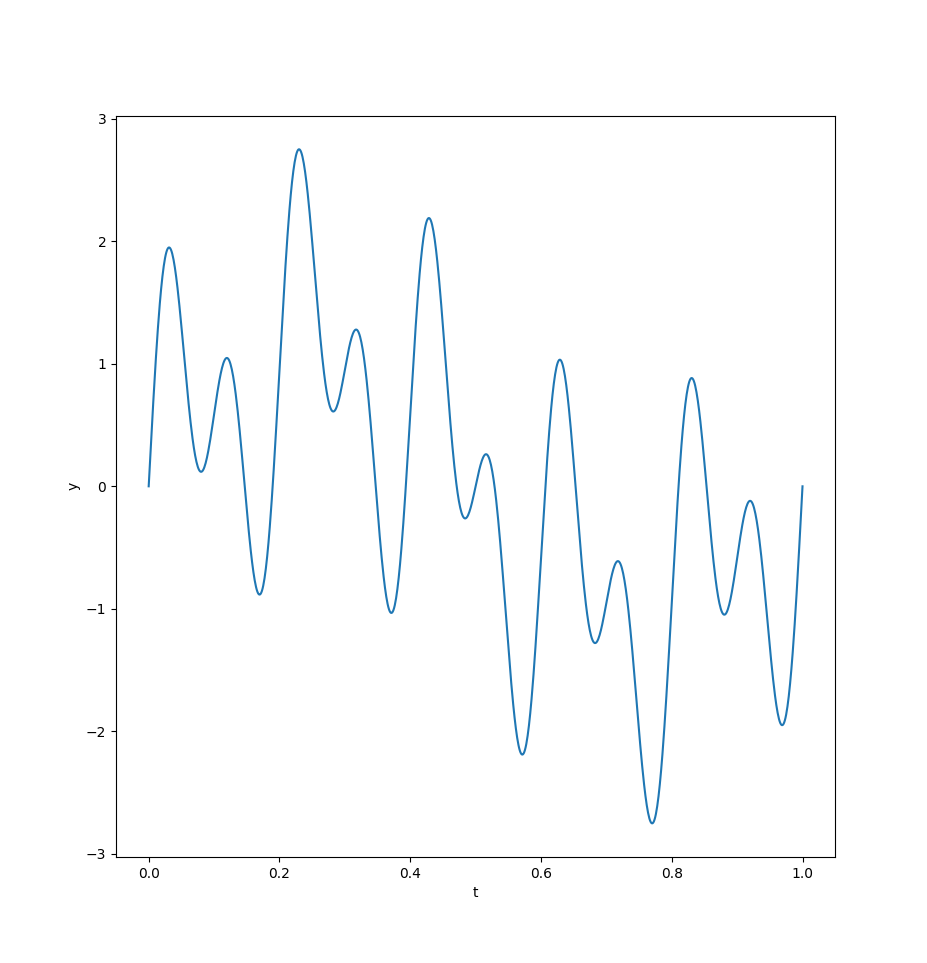
\includegraphics[width=100px]{images/01-what-is-fourier-signal.png}
        \end{column}
        \hspace*{-50px}
        \rightarrow
        \begin{column}{60px}
            \centering
            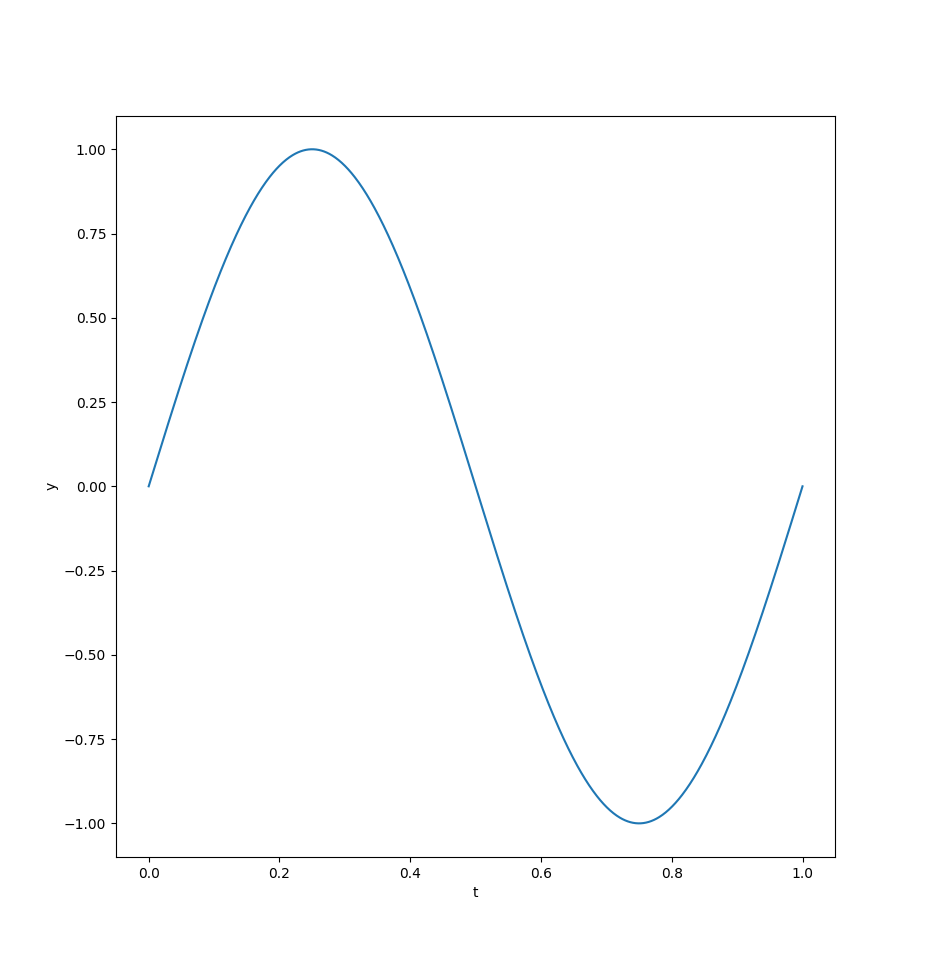
\includegraphics[width=50px]{images/01-what-is-fourier-signal-component-1.png}
            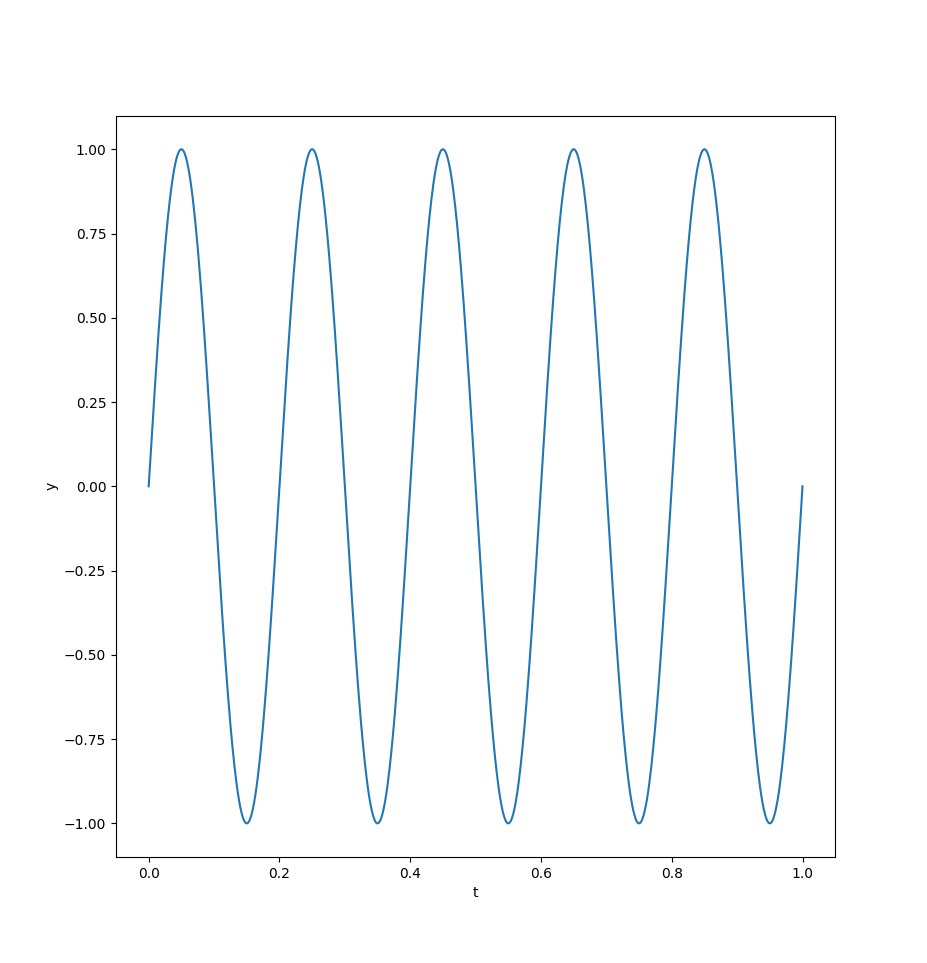
\includegraphics[width=50px]{images/01-what-is-fourier-signal-component-2.png}
            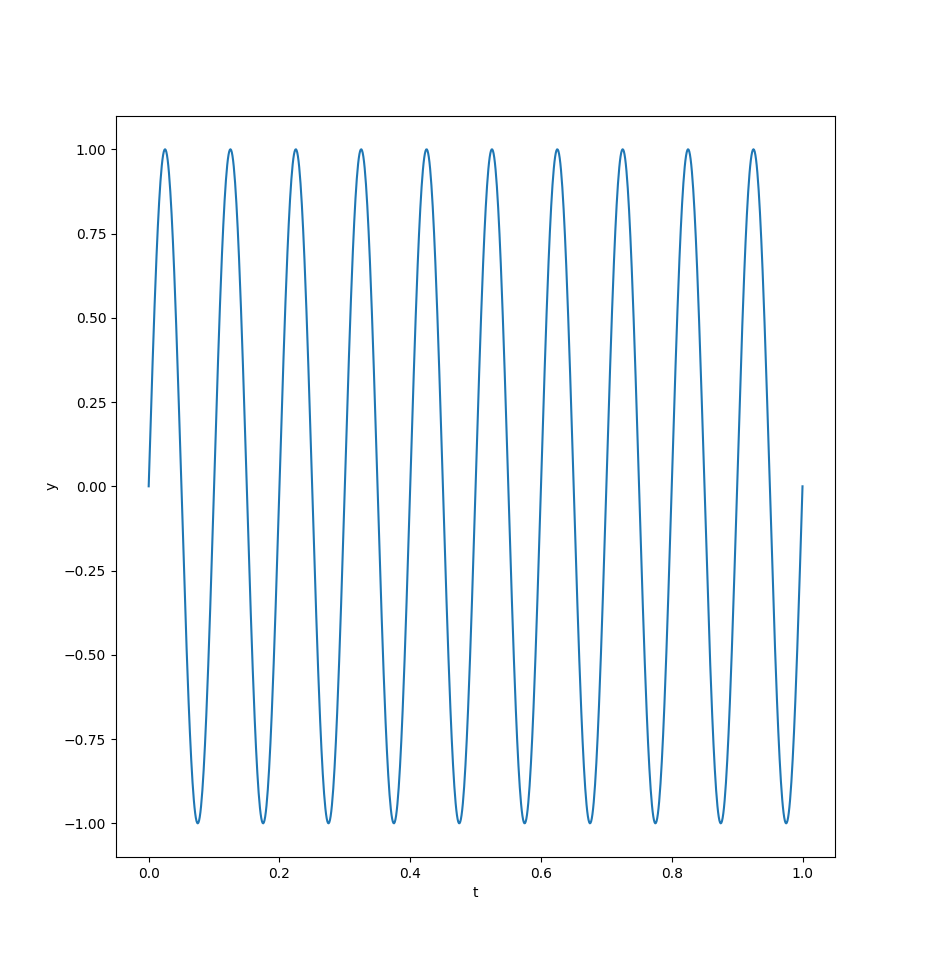
\includegraphics[width=50px]{images/01-what-is-fourier-signal-component-3.png}
        \end{column}
        \hspace*{-40px}
        \rightarrow
        \begin{column}{110px}
            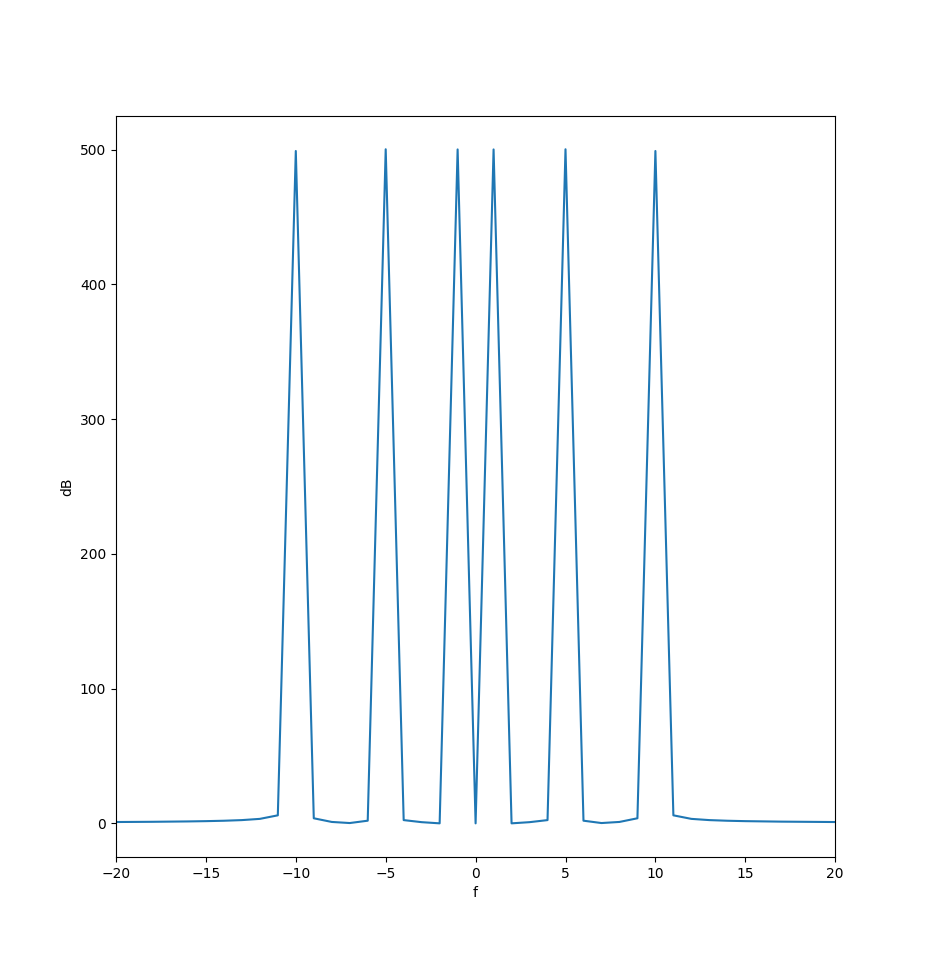
\includegraphics[width=100px]{images/01-what-is-fourier-signal-transform.png}
        \end{column}
    \end{columns}

\end{frame}
